\chapter{Evaluierung}
\label{cha:evaluation}

Dieses Kapitel präsentiert die Ergebnisse der Arbeit. Dabei werden die finalen\linebreak Diagramme und ihre einzelnen Funktionen präsentiert. Innerhalb der Diagramme wird der in den Testfällen beschriebene Datensatz (Abschnitt \ref{sec:impl_tests}) mit einem daraus erstellten linearen Regressionsmodell dargestellt. Nach der Präsentation der Ergebnisse wird überprüft, ob die implementierten Diagramme die Problemstellung erfolgreich lösen. Im Zuge dessen werden auch mögliche Verbesserungen der Bibliothek hervorgehoben. Alle Ergebnisse werden danach zum Ende des Kapitels als Tabelle zusammengefasst.

\section{Präsentation der Ergebnisse}
\label{sec:eval_presentation}

Die wichtigsten Ergebnisse der Arbeit sind die Implementierungen der Diagramme.\linebreak Der Sourcecode der Bibliothek selbst ist auf GitHub unter der Adresse\linebreak \emph{https://github.com/Pystronic/scikit-charts} verfügbar.

\begin{figure}[H]
    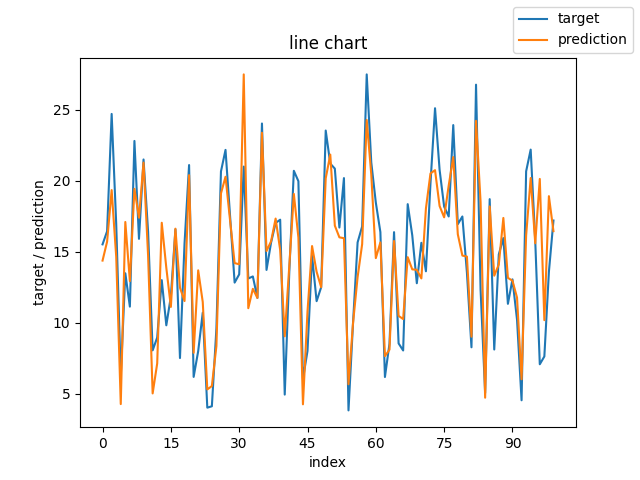
\includegraphics[width=0.5\textwidth]{images/exm_liniendiagramm.png}
    \hfill
    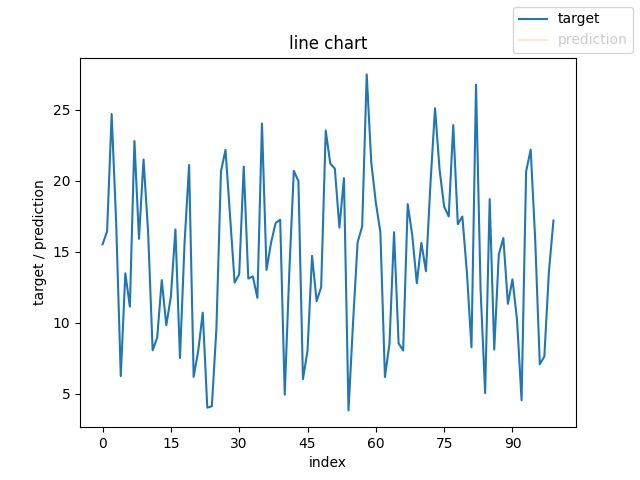
\includegraphics[width=0.5\textwidth]{images/exm_liniendiagramm_interacted.png}
    \caption{Ergebnis des Liniendiagramms und dessen Interaktion}
    \label{fig:eval_line_chart}
\end{figure}

\noindent Das Liniendiagramm konnte mit mit demselben Funktionen wie in HeuristicLab umgesetzt werden. Einzig die Unterscheidung zwischen Test- und Trainingsdaten wird nicht unterstützt. Es kann ohne weitere Konfiguration angwendet werden, um Muster\linebreak basierend auf dem Index in den Zielwerten zu finden. Dieses Muster kann dann mit dem Ergebnissen der Vorhersage verglichen werden. Dabei erweitert das Diagramm die\linebreak Standardimplementierung des Liniendiagramms um das dynamische Ausblenden von Daten über die Legende. Diese Funktion ist in Abbildung \ref{fig:eval_line_chart} ersichtlich. In dieser werden die Vorhersagen zwischen den beiden Darstellungen ausgeblendet.

\begin{figure}[H]
    \centering
    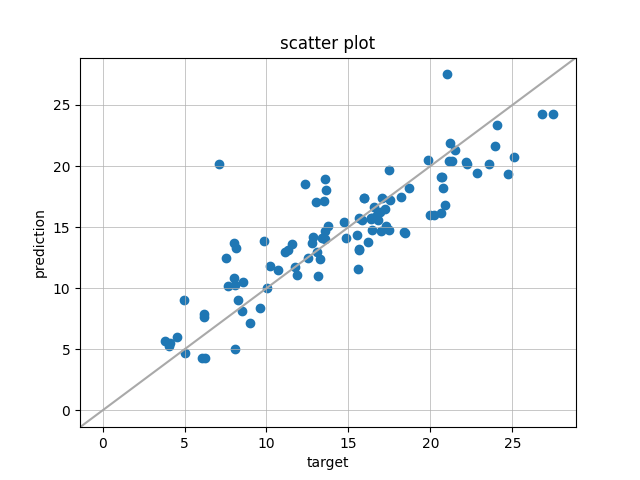
\includegraphics[width=0.5\textwidth]{images/exm_scatterplot.png}
    \caption{Ergebnis des Streudiagramms}
    \label{fig:eval_scatter_plott}
\end{figure}

\noindent Das finale Streudiagramm stellt eine konfigurierte Variante der Standardimplementierung aus Matplot dar. Dabei besitzt das Diagramm standardmäßig ein Gitter, sowie die 45° Linie in der Darstellung. Es ermöglicht Anwender:innen einen schnellen und präzisen Vergleich der Vorhersagen gegenüber den Zielwerten.

\begin{figure}[H]
    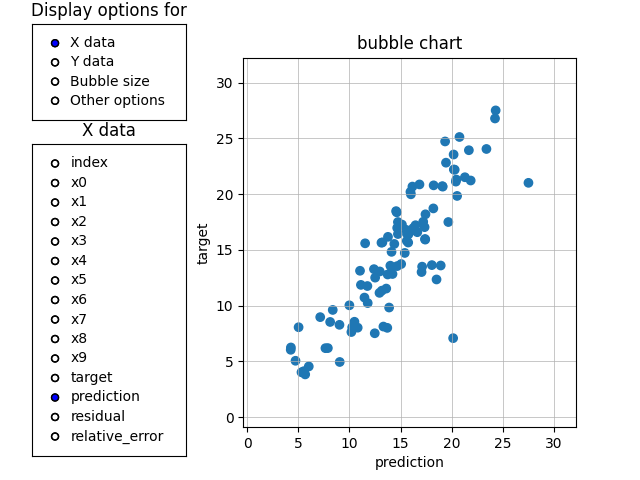
\includegraphics[width=0.5\textwidth]{images/exm_bubblechart.png}
    \hfill
    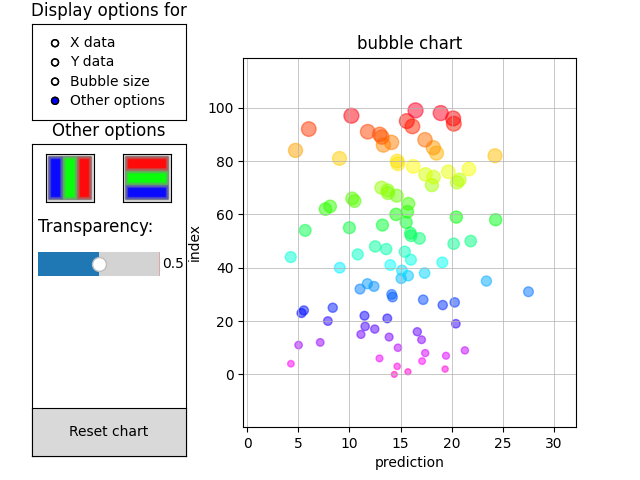
\includegraphics[width=0.5\textwidth]{images/exm_bubblechart_interacted.png}
    \caption{Ergebnis des Blasendiagramms und dessen Interaktionen}
    \label{fig:eval_bubble_chart}
\end{figure}

\noindent Mit der finalen Implementierung des Blasendiagramms wird eine Erweiterung des\linebreak standardmäßigen Streudiagramms zur Verfügung gestellt. Über die Blasengröße ermöglicht das Diagramm den Vergleich dreier Metriken auf einmal. Im Zentrum steht dabei die dynamische Auswahl der Metrik für die einzelnen Achsen und die Blasengröße. Durch diese wird ein interaktiver Vergleich ermöglicht, ohne jedes Mal ein neues Diagramm zu generieren. Die Färbung erlaubt es, die Blasen über die Werte einer Metrik weiter hervorzuheben. Da diese Färbung beim Wechseln der Achsen-Metrik erhalten bleibt, ermöglicht sie es ebenfalls eine vierte Dimension für Vergleiche einzubauen. Mithilfe des Sliders für die Transparenz ist es möglich die Dichte der Datenpunkte zu überprüfen. Dabei werden bei einer hohen Transparenz dichte Punkte durch die Überlappung stärker angezeigt. Zuletzt gibt es noch die Möglichkeit das gesamte Diagramm auf die initialen Werte zurückzusetzen. Das betrifft sowohl für die gesetzten Metriken, als auch die Färbung und Transparenz.

\begin{figure}[H]
    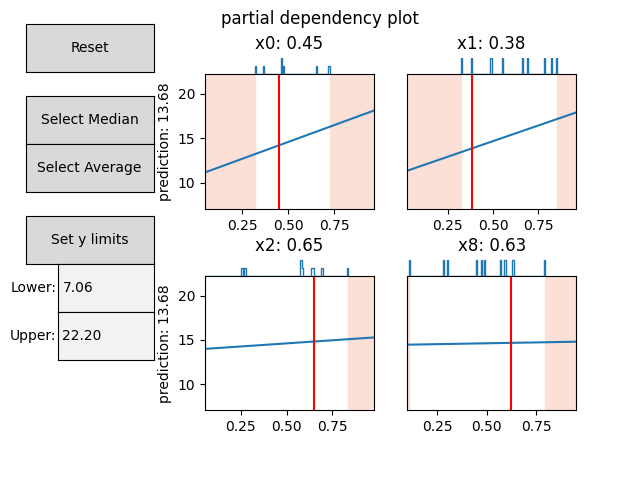
\includegraphics[width=0.5\textwidth]{images/exm_schnittdiagramm.png}
    \hfill
    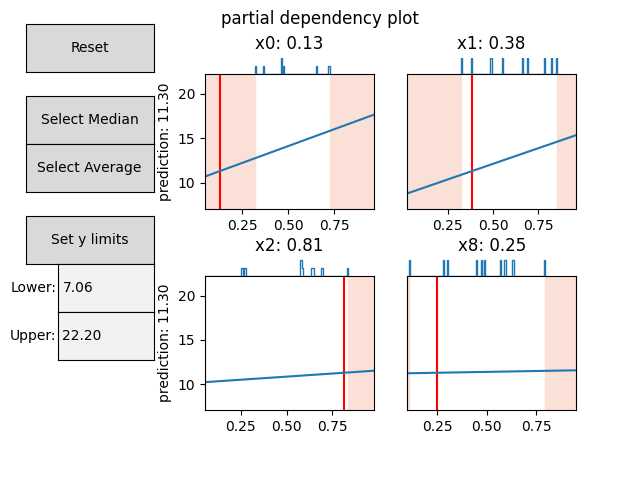
\includegraphics[width=0.5\textwidth]{images/exm_schnittdiagramm_after_moving.png}
    \caption{Ergebnis des Schnittdiagramms und dessen Interaktionen}
    \label{fig:eval_partial_dependency}
\end{figure}

\noindent Das finale Schnittdiagramms ermöglicht es, den Einfluss mehrerer Einflussvariablen\linebreak dynamisch zu analysieren. Dabei werden beim Aufruf des Diagramms die Traningsdaten des in Scikit-learn trainierten Modelles, sowie die Indices der darzustellenden Einflussvariablen übergeben. Der Einfluss der einzelnen Variablen wird daraufhin berechnet und in Feldern dargestellt. Die blaue Linie in der Mitte der Felder zeigt dabei das Verhältnis des Einflusses an. Das Verhältnis ist dabei die Relation zwischen den möglichen Werten auf der X-Achse und den Vorhersagen auf der Y-Achse. Über den einzelnen Feldern ist die Dichte der Werte im originalen Datensatz eingezeichnet. Diese wird als Histogramm dargestellt. Bereiche welche sich nicht im originalen Datensatz befinden, werden in den Felder mit einer roten Färbung hinterlegt. Die rote vertikale Linie der Felder zeigt den aktuell gewählten Wert für eine Variable an.\\\\
\noindent Sowohl die berechnete Vorhersage am Beginn der Reihen, als auch das dargestellte Verhältnis ist abhängig von den aktuell gewählten Werten. Vorhersage und\linebreak dargestellter Einfluss werden beim Verändern der Auswahl automatisch aktualisiert. Die Auswahl eines Wertes erfolgt durch das Verschieben der Linie mithilfe der Maus. Alternativ kann der gewählte Werte für alle Einflussvariablen über die Knöpfe in der Seitenleiste gesetzt werden. In Abbildung \ref{fig:eval_partial_dependency} ist der Unterschied vor und nach dem Verschieben ersichtlich. In der Seitenleiste ist es ebenfalls möglich, den Wertebereich für die\linebreak Y-Achse anzupassen. Die Anzahl der dargestellten Spalten, sowie die Anzahl an generierten Werte, pro Variable können nur beim Aufruf der Funktion konfiguriert werden. Es ist außerdem möglich, die Seitenleiste beim Aufruf des Diagramms zu deaktivieren.

\pagebreak

\subsection{Ergebnisse außerhalb der Aufgabenstellung}
\label{subsec:eval_other_results}

\noindent Neben den Diagrammen wurde auch noch weitere Ergebnisse erzielt. Die Implementierung der Metriken kann auch außerhalb der Bibliothek angewandt werden. Dasselbe gilt für die geteilten Hilfsklassen der einzelnen Diagramme. Diese können bei der Erstellung eigener interaktiver Visualisierungen von Anwender:innen genutzt werden. Bei diesen Hilfsklassen handelt es sich um Wrapper für Matplot UI-Elemente. Diese\linebreak vereinfachen die Platzierung und Erstellung der Elemente in einem Diagramm. Außerdem werden auch erweiterte interaktive Elemente, welche nicht standardmäßig existieren, zur Verfügung stehen.

\section{Gegenüberstellung der Ergebnisse mit der Problemstellung}
\label{sec:eval_problemstellung}

In der Problemstellung (Abschnitt \ref{sec:Problemstellung}) werden Anforderungen an Bibliotheken zur\linebreak Visualisierung von Regressionsmodellen definiert. Dabei können drei konkrete\linebreak Anforderungen zusammengefasst werden:
\begin{enumerate}
    \item Keine Notwendigkeit von spezifisches Wissen.
    \item Einfache Integration der Diagramme.
    \item Dynamische Analysen durch Interaktivität.
\end{enumerate}

\vspace{\baselineskip}

\noindent Punkt 1 wird mit Einschränkungen erfüllt. Scikit-chart abstrahiert Matplot über den Aufruf des Diagramms. Es kann jedoch notwendig sein einige Einstellungen zu treffen, um Interaktivität der Diagramme zu aktivieren. Diese benötigen Matplot spezifisches wissen. Das ist vor Allem in Jupyter Notebook der Fall. Die notwendigen Schritte sind jedoch in Abschnitt \ref{subsec:impl_backend} beschrieben.\\\\
\noindent Punkt 2 wird von der Bibliothek erfüllt. Durch die Implementierung über Matplot können die Diagramme auf unterschiedlichen Plattformen integriert werden. Drei der Vier Diagramme können Regressionsmodelle unabhängig der verwendeten Bibliothek\linebreak darstellen. Einzig das Schnittdiagramm besitzt die Einschränkung auf ein mit Scikit-learn trainiertes Modell. Der Aufruf der Diagramme selbst, ist von den Funktionen in Scikit-learn inspiriert. Durch die ähnliche Reihenfolge der Argumente können sich Anwender:innen von Scikit-learn leichter in die Bibliothek einfinden. Zuletzt unterstützt die konsequente Verwendung von eingebetteter Dokumentation sowie von Typinformationen die Anwender:innen bei der Integration.\\\\
\noindent Punkt 3 wird über Blasendiagramm und Schnittdiagramm unterstützt. Beide Diagramme ermöglichen eine interaktive Analyse eines Regressionsmodells sowie des dazugehörigen Datensatz. Die Interaktivität vereinfacht es dabei mögliche Zusammenhänge zwischen den Daten zu erkennen. Liniendiagramm und Streudiagramm erfüllen diesen Punkt jedoch nicht, wegen ihrer geringen Interaktivität.

\section{Gegenüberstellung der Ergebnisse mit der Zielsetzung}
\label{sec:eval_zielvorgabe}

Die Zielsetzung (Abschnitt \ref{sec:Zielsetzung}) wurden umgesetzt. Die Funktionalitäten aus HeuristicLab wurden jedoch nicht komplett übernommen. Die Bibliothek unterstützt\linebreak das Sammeln der Metriken, welche in aus HeuristicLab identifiziert wurden. Die Implementierungen der Diagramme orientieren sich an HeuristicLab, besitzen jedoch einige Einschränkungen. Konkret fehlen Funktionalitäten bei Blasendiagramm und Schnittdiagramm. Beim Blasendiagramm sind es die Auswahl von Datenpunkten, sowie das Färben und Verstecken der gewählten Punkte. Des Weiteren gibt wurde der Jitter sowie die weitere Anpassung der gewählten Blasengröße nicht implementiert. Beim Schnittdiagramm fehlt die dynamische Auswahl der Einflussvariablen sowie die dynamische Änderung der Spaltenanzahl. Es fehlt ebenfalls das Setzen der Variablenwerte auf eine gewisse Zeile im Datensatz. Bei den restlichen Punkten der Zielsetzung gab es keine Einschränkungen. Mithilfe von Poetry, kann aus dem Projekt ein Python-Paket gebaut werden. Dadurch kann die Bibliothek entweder systemweit installiert oder für bestimmte Projekt hinzugefügt werden. Die Unterstützung von Scikit-learn wurde sogar überfüllt, da Liniendiagramm, Streudiagramm und Blasendiagramm beliebige Modelle unter-stützen. Die Integration in Jupyter Notebooks wurde ebenfalls getestet und notwendige Konfigurationen in Abschnitt \ref{subsec:impl_backend} beschrieben.

\section{Mögliche Verbesserungen der Bibliothek}
\label{sec:eval_improvements}

Die bestehende Implementierung unterstützt alle notwendigen Anforderungen.\linebreak Trotzdem könnten noch verschiedene Verbesserungen getroffen werden, um den Wert der Bibliothek für Anwender:innen zu erhöhen. Diese Verbesserungen umfassen Usability, Performance, Stabilität und Flexibilität.\\\\
\noindent Die möglichen Verbesserungen in der Usability auf die Interaktion mit den einzelnen Diagrammen. Bei der interaktiven Legende, den RadioButtons und roten Linie im Schnittdiagramm sollte der Cursor auf eine Hand geändert werden. Dadurch wird die Interaktivität dieser Elemente impliziert. Weiters könnte das Layout der Diagramme verbessert werden. Dabei sollte die Seitenleiste verkleinert werden, was eine eigene Drop-Down-Implementierung erforderlich macht. Zuletzt könnte noch die Skalierung in den Diagrammen verbessert werden. Aktuell skalieren Textgrößen und die Größe der UI-Elemente nicht korrekt mit der Fenstergröße.\\\\
\noindent Für eine bessere Performance können drei Punkte in Betracht gezogen werden. Zuerst könnte eine Alternative zu Pandas-Dataframes für die Speicherungen der Metriken verwendet werden. Das liegt daran, dass der Zugriff auf einen Dataframe ist langsamer ist als die Verwendung von Numpy-Arrays. Weiters könnte auf die Verwendung eines Dataframes im Liniendiagramm und Schnittdiagramm verzichtet werden. Diese benötigen zur Darstellung nur einen Teil der Metriken. Eine weitere mögliche Verbesserung könnte auch die Implementierung von \emph{blitting}\footnote{https://matplotlib.org/stable/tutorials/advanced/blitting.html} darstellen. Dabei werden alle statischen Elemente einmalig gezeichnet und als Bild abgespeichert. Bei jeder Aktualisierung\linebreak werden nur noch das gespeicherte Bild und die aktualisierten Elemente gezeichnet. Die letzte mögliche Verbesserung ist bei der Berechnung der partial dependence möglich. Diese stellt aktuell die größte Einschränkung im Schnittdiagramm dar. Eine schnellere Berechnung würde die Anzahl der darstellbaren Einflussvariablen erhöhen. Dafür könnte entweder die Implementierung in Scikit-learn auf Verbesserungen geprüft werden oder eine eigene Implementierung erstellt werden. Die eigene Implementierung hätte den Vorteil, dass sie genau den Anforderungen von Scikit-charts entsprechen würde. Dafür würde diese ebenfalls den Wartungsaufwand der Bibliothek erhöhen.\\\\
\noindent Die Verbesserungen der Stabilität umfassen vor Allem eine höhere Anzahl an automatisierten Tests. Diese könnten mögliche Fehler bei den Diagrammen genauer vorbeugen. Außerdem sollten für zur Validierung der Darstellung Visual-Regression Tests\linebreak \parencite{VisualRegression} in Erwägung gezogen werden. Dabei ein Bild eines korrekt dargestellten Diagramms mit neueren Bildern der Diagramme verglichen. Die Testfälle stellen dadurch die konsistente Darstellung der Daten sicher. Als ein weiterer Punkt sollte noch geprüft werden, ob die fehlende Rückgabe des Diagramm-Objektes zu Problemen während der Ausführung führen kann. In den aktuellen, kurzen Tests konnte das noch nicht eindeutig festgestellt werden. Zuletzt könnten noch genauere Validierungen für die Argumente von Funktionen durchgeführt werden. Dies würde vor allem beim Hinzufügen neuer Parameter notwendig und ermöglicht es Laufzeitfehler besser vorbeugen.\\\\
\noindent Als letzter Punkt könnte noch die Flexibilität der Bibliothek verbessert werden. Dafür würden mehr Parameter in den Hilfsklassen hinzugefügt werden. Diese sollten die Konfiguration der optionalen Parameter von Matplot ermöglichen. Dadurch wird die Verwendung für eigene Diagrammimplementierungen durch Anwender:innen verbessert werden. Liniendiagramm und Streudiagramm könnten außerdem allgemein definiert werden, um beliebige Daten der Anwender:innen damit darzustellen. Zuletzt könnte das Blasendiagramm erweitert werden, sodass Anwender:innen eigene Metriken definieren und\linebreak vergleichen können. Dadurch würde sichergestellt werden, dass durch die beschränkten Metriken keine Einschränkungen für Anwender:innen entstehen.

\section{Reflexion}
\label{sec:ausblick}

Aus persönlicher Sicht ist das Ergebnis der Bachelorarbeit zufriedenstellend. Die Durchführung der Arbeit hätte jedoch besser laufen können. Trotz einiger privater Herausforderungen wurde die verfügbare Zeit eher suboptimal genutzt. Die Arbeit könnte dementsprechend noch weiter ausgebaut werden. Inhaltlich kann die Arbeit jedoch trotzdem als Einstieg in verschiedene Themen genutzt werden. Sie bietet Leser:innen grundlegendes Wissen über Regressionmodelle und Datenanalyse. Das Hauptthema stellt\linebreak jedoch eindeutig die Visualisierung dar. Im Bezug darauf kann die Bibliothek als ein Einstieg in die Verwendung von Matplot verwendet werden. Dabei unterstützen die aufgelisteten Probleme, welche bei der Nutzung der Bibliothek entstehen können. Im Bezug\linebreak auf die Implementierung wurde zwar die grundlegende Zielsetzung erfüllt,\linebreak dennoch existiert unausgeschöpften Potenzial. Somit liegt es an der Zeit nach der Arbeit, dieses Potenzial weiter auszuschöpfen. 

% Notes:
% - Probleme / Herausforderungen beim Entwickeln:
%   - Jupyter notebook -> Diagramme werden zweimal angezeigt -> Jupyter zeigt generierte matplot-figures automatisch an -> Lösung: Strichpunkt am einde von Funktionsaufruf oder rückgabewert abspeichern -> Kein .show aufruf notwendig

% Aufgaben:
% - Feinschliff
%   - Konsequentes Großschreiben von Bibliotheksnamen
%   - Fehler ausbessern + Schreibweise prüfen
%   - References zu Biliotheken als Bib-Reference zu Software
%   - Literaturverzeichnis fixen
%   - Prüfen wegen Emph, ob überall gesetzt